\section{Topic Tree}

The topic tree feature will be examined based on a framework to determine how well the implemented feature has achieved its intended purpose and its functionality. \\

Therefore the analysis includes four sections:\\
\begin{itemize}
    \item Functional Requirements - does the system fulfil the functional requirements set out in the project approach?
    \item Non-functional requirements - how well does the system achieve the non functional requirements including performance and accessibility
    \item Scalability and Efficiency - how well does the feature perform with many, many topics and topic groups?
    \item Feedback from potential users of the feature - what do users such as lecturers, tutors and students think about the feature and how could it be improved?
\end{itemize}

\subsection{Functional requirements}
The functional requirements of the feature were analysed for completedness. Each functional requirement has a priority attached to it, and the functionality of the system was assessed against this priority. \\

In total, 15 requirements out of 19 were fully completed. 1 high requirement, 1 medium requirement and 1 low requirement were not completed at all. 9 high requirements, 5 medium requirements and 1 low requirement were completed. \\

The following explains the requirements that were not completed and why they were not completed.\\
\\
\textbf{Users can search for specific resources - High Priority} \\
Currently the topic tree feature allows users to search through the topic tree for specific topics, but does not allow users to search through the entire topic tree for a specific resource. This is because topic resources are already grouped by topic, and there was no need to have to search the entire topic tree for a specific resource. Also, tags were added as a feature where users can specify different synonyms for a topic, improving searchability. Topic resources is also commonly given generic names, such as "Lecture Slides". This is not descriptive of the content, and would have proved resource searchability difficult. \\
\\
\textbf{Users can delete a topic group that they've created - Medium Priority}\\
Users can currently create topic groups, but cannot delete them. This is due to integration issues found with deleting topics, as topic groups are an integral part of the entire system. Deleting topic groups could create database integrity issues, and there was not enough time to fix these issues.\\
\\
\textbf{Users can export data from topics and course material - Low Priority} \\
This requirement was classed low priority as the system was designed to be the only learning management system for an entire faculty or university. Exporting data from topics and course material would have proved useful for exporting into another learning management system, but there was again not enough time to implement this feature either.\\

\subsection {Non functional requirements}

The following details the analysis undertaken to examine the accessibility, security and performance of the feature. 

\subsection {Performance}

Performance of the system could be improved, with the main topic tree graph view loading a little slowly. Google Lighthouse was used to analyse performance, and performance differs depending on the database server used i.e. if a remote server was used, the topic tree takes longer to load the graph.\\

Google Lighthouse is a tool used to measure page performance and accessibility, and gives a score out of 100 after running its tests. It waits until there is no more movement on the graph and measures the time taken, however the page is interactive before movement stops on the graph due to nodes slowly moving outwards from where they loaded.\\

\begin{figure}[h!]
    \centering
    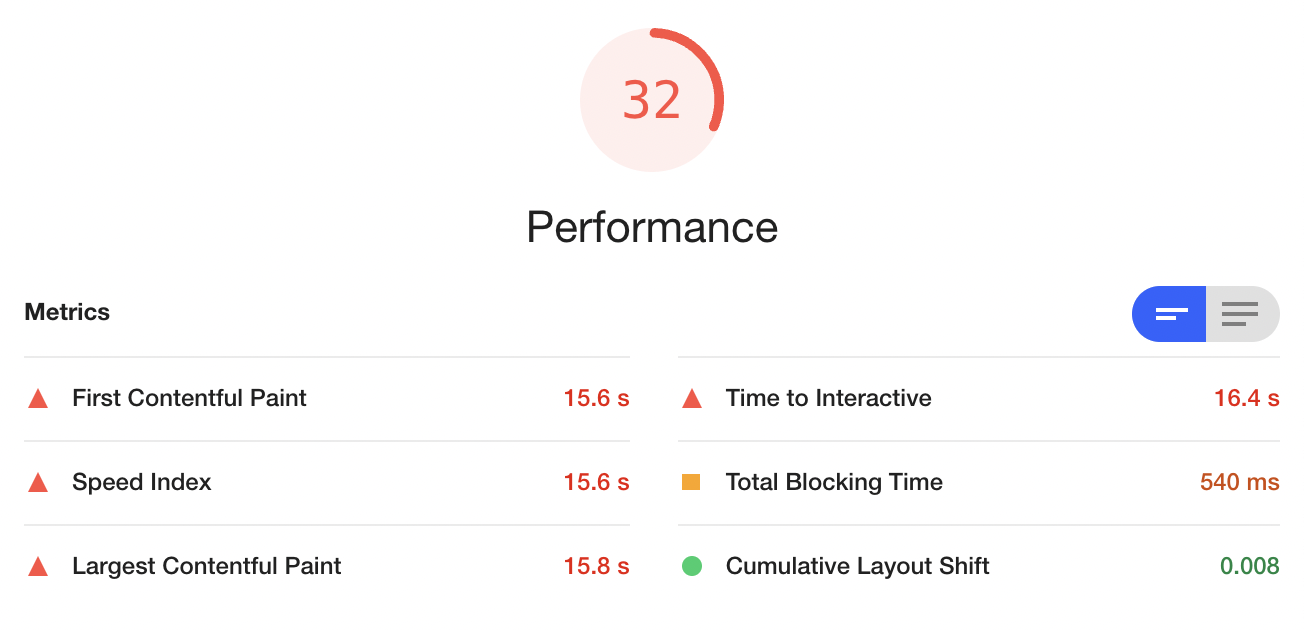
\includegraphics[scale=0.4]{topic-tree-performance}
    \caption{Performance report of the topic tree}
\end{figure}

As shown in the report, a score of 32/100 was given for the topic tree's performance. Restructuring of the database and less API requests are strategies that can be used to improve the performance of the topic tree, as well as a different graphing library as d3 is not an optimised library for handling graphs.\\

\subsection{Accessibility}
Accessibility of the feature is good, as the Chakra UI library was used to ensure that alt and aria tags were used. Colour contrast of the feature could be improved, but is still quite good with contrasting blue and white colours used. \\

\begin{figure}[h!]
    \centering
    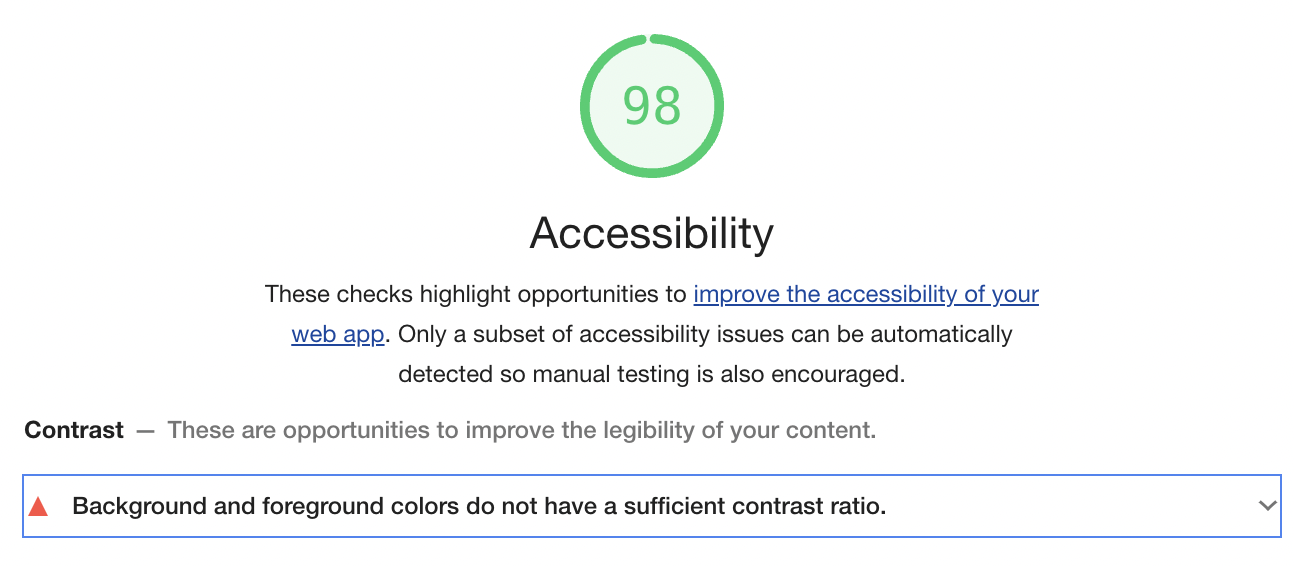
\includegraphics[scale=0.4]{topic-tree-accessibility}
    \caption{Accessibility report of the topic tree}
\end{figure}

A score of 98 was achieved for accessibility. Google Lighthouse accesses tags and HTML elements used, as well as contrast ratios to assess accessibility.\\

\subsection{Scalability Testing}

This section focuses on how well the feature copes against tens and hundreds of topic groups and a large amount of data. As the feature will be used with many, many topic groups, scalability testing is performed to ensure the feature is usable.\\

To assess the feature, each topic group will contain 3 topics to simulate a real world topic group. The feature will be tested with 3, 5, 10, 20, 50, 100, and 300 topic groups. The School of CSE currently runs around 100 courses, and so as this topic tree is designed to be used by a faculty or school, 300 topic groups is the limit that will be tested. Ideally, disciplines will be implemented in the future which will create separate topic trees for each school or faculty. \\

Each test will be assessed by measuring the performance using Google Lighthouse i.e. the time to finish loading the website. \\
The user experience will also be assessed, with comments made after each test referring to whether managing the number of topics is efficient or not.

\textbf{Results}

\begin{center}
\begin{tabular}{||c c||} 
 \hline
 Number of Topic Groups & Time Taken to Interactive (sec) \\ [0.5ex] 
 \hline\hline
 3 & 3.13 \\ 
 \hline
 5 & 3.16 \\
 \hline
 10 & 3.20 \\
 \hline
 20 & 3.43 \\
 \hline
 50 & 6.05 \\ 
 \hline
 100 & 10.11 \\
 \hline
 300 & 26.47 \\ [1ex] 
 \hline
\end{tabular}
\end{center}

As shown in the above results, some issues arise with more than 50 topic groups. The performance is quite good but can be significantly improved, especially when there are more than 50 topic groups. According to a BBC article on Nordstorm, a popular shopping website, they believe a page load time of 2.5 seconds or less strikes a good balance between functionality and speed. By minimising the amount of data and database requests needed to load the feature, the speed of the topic tree can be dramatically improved.\\

Up to 20 topic groups are also shown on the graph very well, as shown in the screenshot below.
\begin{figure}[h!]
    \centering
    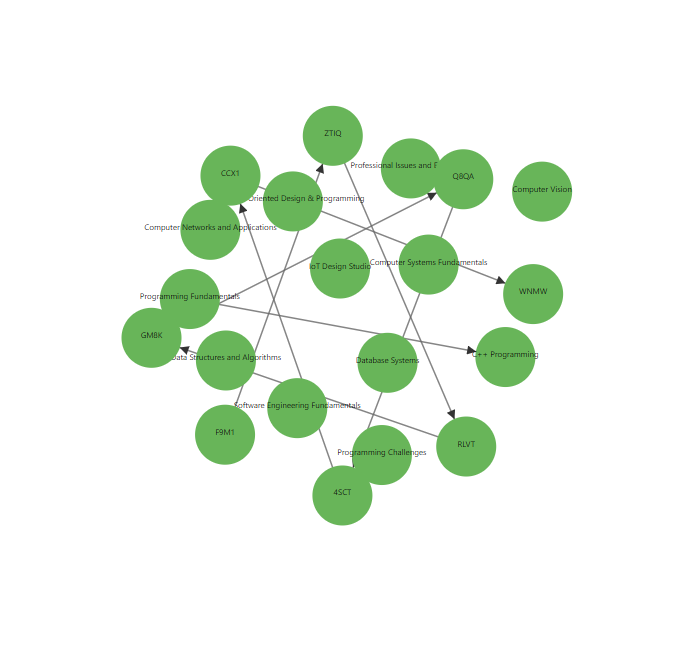
\includegraphics[scale=0.4]{20}
    \caption{20 topic groups on the topic tree}
\end{figure}

However, once 50 or more topic groups are shown, the topic groups start to cluster together. This makes it quite difficult for users to navigate around the topic tree, as shown below as well.

\begin{figure}[h!]
    \centering
    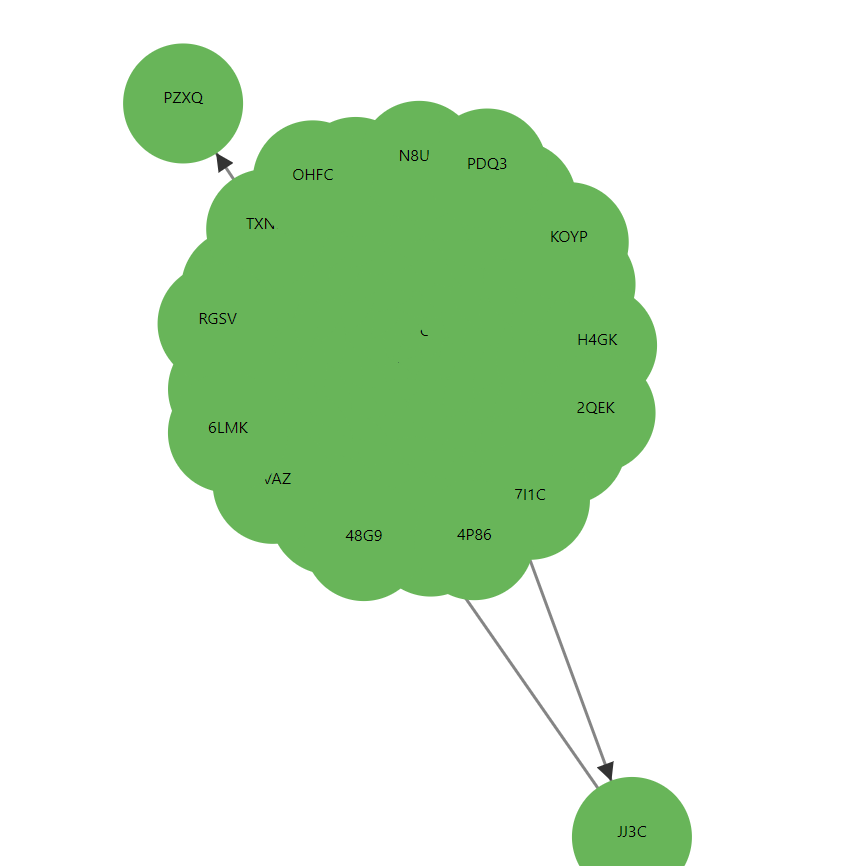
\includegraphics[scale=0.4]{100}
    \caption{100 topic groups on the topic tree}
\end{figure}

The issue is then accelerated with more and more topic groups displayed on the topic tree as well.

\begin{figure}[h!]
    \centering
    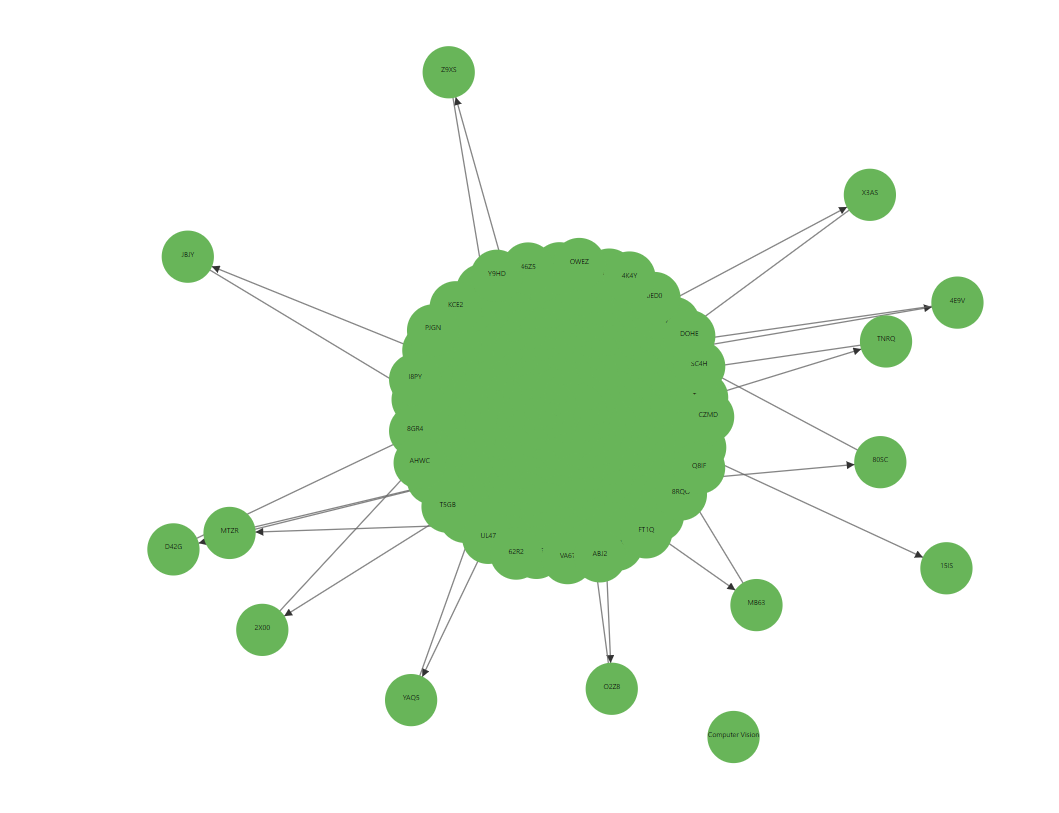
\includegraphics[scale=0.4]{300}
    \caption{300 topic groups on the topic tree}
\end{figure}

This can be improved by altering the force algorithm used to separate the nodes, which was designed by the d3 module that this feature uses to display the graph. 

\subsection{Feedback from Potential Users}
Feedback from students, tutors and lecturers have been collected to analyse the user experience of the system and what could be improved. \\

\textbf{Audience} \\

Feedback was collected from a range of fields including:\\
\begin{itemize}
    \item Computer Science and Engineering
    \item Humanities and Languages 
    \item Business and Economics 
\end{itemize}

This range of different areas provides context on how usable the feature would be in their subject area or faculty, and also provides a diverse range of users.\\

\textbf{Questions} \\
These users were asked various questions before a demonstration of the feature, and then asked more questions after the demonstration as well. The questions are as follows:\\
\textbf{Prior to Demonstration}
\begin{enumerate}
    \item What learning management systems have you used previously?
    \item (Academics only) Have you experienced a situation where you have tried to reuse content? If so, what was it?
\end{enumerate}

People from UNSW all answered the first question with Moodle and some answered WebCMS. One user from the University of Sydney answered Canvas, as they use a different learning management system.\\
Academics from the school of Computer Science and Engineering at UNSW answered the second question with "Yes", and most have explained that it was quite difficult having to create new content for the same topic in their courses. However, academics in Humanities and Languages explained that it was very easy to reuse course content in Moodle, as they only need to create a new offering of the course and have no need to reuse content from other courses.\\

\textbf{After Demonstration}
\begin{enumerate}
    \item Is the system easy to use? What UI issues did you have with it?
    \item (Academics Only) Would you use the system to help organise content better?
    \item Is the terminology of the system such as topics and topic groups easy to understand?
    \item Would you use the graph or list view of the topic tree more?
    \item What are some positive aspects of the topic tree?
    \item What could be improved?
    \item Do you have any final comments or questions?
\end{enumerate}

Most users commented that the system is quite easy to use, however there are some UI issues with the system. Most also agreed that it was quite difficult to see what the topic group was when expanded into their individual topics. There were also various small UI issues throughout the feature, but these did not affect the functionality or the ease of use of the topic tree significantly. \\

Many academics from the faculty of Computer Science and Engineering commented that the system would be extremely useful for managing their courses, as it allows reusability of content and specific topics can be set as prerequisites eg. Git can be set as a prerequisite for COMP6080 instead of having to reteach it.\\

However, academics from the faculty of Languages and Arts commented that they would have little use of the system in helping them organise content better, as they were so used to using Moodle which allows an easy way to offer the same course in a different year. As the content is quite linear i.e. the first topic must be completed before attempting the second topic, etc., the system may be of better use for Computer Science and Economics for example instead where the prerequisite topic tree is more complicated.\\

Many users also responded that they would rather rename 'topic groups' to 'courses' instead, to allow easier use of the system and faster adaptability of the system. However, other users also commented that this may not be an issue as there are many terms within university that are confusing to both students and academics as well such as "course", "major", and "offering".\\

Similar trends were observed where users who would use the system to its full potential i.e. users from the Computer Science faculty, would use the graph view more than the list view more. However, academics from the School of Languages and Arts would prefer to use the list view. One user responded that it was good to have an option to use either as when looking for a course, it is faster to use the list view instead of the graph view but when looking at topics overall, the graph view proves more useful.\\

Many users found the structure of Content, Practice, Preparation and Assessment quite useful, as it can fit many learning models well. The various features such as searching the topic tree and adding tags to various topics also proved useful. Accessibility was another positive aspect of the topic tree, but the algorithm that picks colours to distinguish the groups of topics when expanded sometimes picks colours that are inaccessible. 

Finally, some academics commented that a permission system is needed, as especially in faculties such as Arts and Economics, lecturers tend to not share content with each other due to copyright issues. As all topic groups would be shown on the topic tree, this would be a major issue without a permissions system available.\\

Overall, the feedback of the system was positive and most academics and tutors agreed that the topic tree feature would help create more structure to content and improve the reusability of coursework at university.\\

\textbf{Limitations}
There are various limitations with this structure of the survey, where a demonstration is shown and then questions are asked. A usability test would have made it easier to gauge the UI issues of the system, however due to the limited amount of time academics had to complete the survey, a demonstration structure was adopted instead. UI issues with the feature were still observed, and the feedback given was of high quality.
